\documentclass[12pt]{extarticle}
\usepackage[utf8]{inputenc}
\usepackage[english]{babel}
\usepackage{amsmath}
\usepackage{amsfonts}
\usepackage{amssymb}
\usepackage[margin=12mm,includefoot]{geometry}
\usepackage[hidelinks]{hyperref}

%Header and Footer Stuff
\usepackage{fancyhdr} 
\pagestyle{fancy}
\fancyhead{}
\cfoot{}
\rfoot{\thepage}
\renewcommand{\headrulewidth}{0pt}
\renewcommand{\footrulewidth}{0.1mm}

%Bullet
\renewcommand{\labelitemi}{-}
\renewcommand{\labelitemii}{$\circ$}
\renewcommand{\labelitemiii}{}

%Image
\usepackage{graphicx}
\usepackage{float}
\usepackage{caption}
\usepackage{subcaption}

\date{}
\author{Francesco Buttafuoco}


\newcommand{\hmwkTitle}{Synthesis and optimization of digital systems} % Assignment title
\newcommand{\hmwkDueDate}{2015/2016} % Due date
\newcommand{\hmwkAuthorName}{Francesco} % Your name
\newcommand{\spaceBreackLine}{3mm} 

\title{
\vspace{2in}
\textmd{\textbf{\hmwkTitle}}\\
\normalsize\vspace{0.1in}\normalsize{\hmwkDueDate}\\
\vspace{3in}
}


\begin{document}

\maketitle
\thispagestyle{empty}
\newpage

\tableofcontents	

\thispagestyle{empty}
\cleardoublepage
\setcounter{page}{1}


\section{Introduction}

\subsection{Microelectronic Economics}
\begin{itemize}
\item \textbf{Fixed Costs}: Design
\item \textbf{Variable Costs}: Energy for manufacturing, material needed
\end{itemize}
The higher the integration level, the better and cheaper the final product, true for high-volume production. In fact volume recaptures manufacturing and designs cost.
\bigskip \\
For applications that do not enjoy high-volume (ASICs), other factors matter: reduction of design time (and cost) and quality of the design.
\bigskip \\
\textbf{Variability}: variation of the geometry of transistor that introduce error about speed because \textit{lithography} is not so precise and do not allow to create a good channel in the transistors.

\subsection{CAD}
\textbf{CAD} (Computer-Aided Design) allow to:
\begin{itemize}
\item Reduces design time
\item Multi-objective optimization (area, speed, power)
\item Large scale design management
\end{itemize}
CAD tools reduce time to market, reducing the \textit{fixed cost}. Moreover you can also reduce the \textit{variable cost} optimizing the area and using less silicon.

\subsection{Integrated Circuit Design Styles}
\begin{figure}[H]
	\centering
	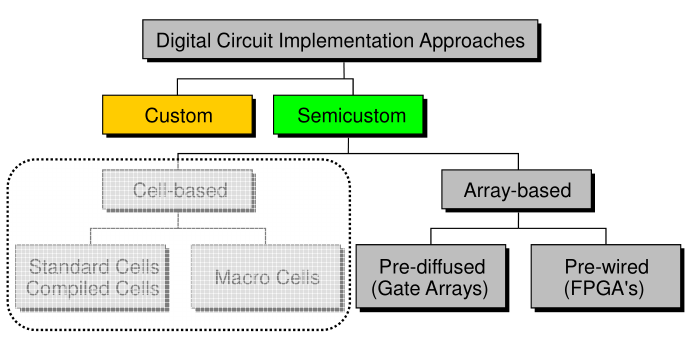
\includegraphics[height=90 mm]{./Cap1/Images/Image01.png}
	\caption[Optional caption]{Integrated Circuit Design Styles}
	\label{fig:ICDS}
\end{figure}
The \textbf{custom} approach (design \textit{by hand}):
\begin{itemize}
\item Functional and physical design are hand-crafted operations
\item Extensive effort (and cost) to optimize each feature
\item Typical of \textit{critical portions} of high-performance designs
\end{itemize}
The \textbf{Semi-custom} approaches
\begin{itemize}
\item Limited number of circuits primitives that allows designers to leverage “optimized” primitives and focus on their \textit{interconnection}
\item Semi-custom design are the big majority of digital design
\end{itemize}
Type of \textbf{Semi-custom} approaches:
\begin{itemize}
\item \textbf{Cell-based}: use  standard cells  or  macrocells  (larger functions)
\begin{itemize}
\item \textbf{Standard cells}: Designed once and highly optimized, stored into a library
\item  \textbf{Macrocells}: Primitives generated by  module generators, ynthesized layout thanks to predefined structures (SRAMs, ROMs)
\end{itemize}
\item \textbf{Array-based}:  Exploit the use of a matrix of uncommitted components which are eventually personalized and connected
\begin{itemize}
\item \textbf{Re-diffused arrays}: Personalization by metalization/contacts (MPGAs).
\item \textbf{Pre-wired arrays}: Personalization on the field (FPGAs).
\end{itemize}
\end{itemize}

\subsection{Microelectronic Design}
Three major tasks (repeated at different \textit{Abstraction levels}):
\begin{itemize}
\item \textbf{Conceptualization and modeling} (Description): Hardware Description Languages (HDL)
\item \textbf{Synthesis and optimization}: Create the structure
\item \textbf{Validation}: Check for correctness
\end{itemize}
\textbf{Models} can be classified in terms of
\begin{itemize}
\item \textit{Abstraction levels}
\begin{itemize}
\item \textbf{Architectural-level} (or RT-level): Operations implemented by
resources.
\item \textbf{Logic-level}: Logic functions implemented by gates.
\item \textbf{Geometrical-level} (or Circuit-level): Circuit implemented by electronic device
\end{itemize}
\item \textit{Views}
\begin{itemize}
\item \textbf{Behavioral} view: Abstract function.
\item \textbf{Structural} view: An interconnection of parts.
\item \textbf{Physical} view: Physical objects with size and positions.
\end{itemize}
\end{itemize}
\begin{figure}[H]
	\centering
	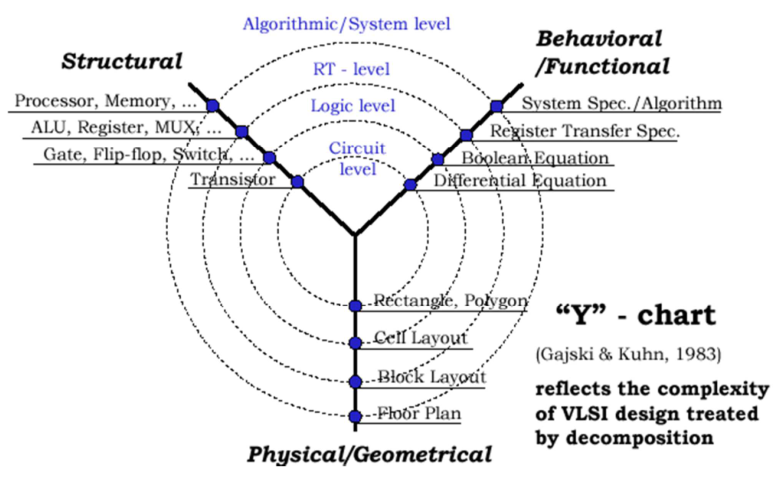
\includegraphics[height=90 mm]{./Cap1/Images/Image02.png}
	\caption[Optional caption]{Y chart}
	\label{fig:Ychart}
\end{figure}
In the Figure \ref{fig:Ychart} the axis represent the \textit{Abstraction levels}, the circles the \textit{Views}.\\
It shows the same \textit{Abstraction levels} at different \textit{Views} and vice versa.\\
The \textbf{synthesis} is the switching from Behavioural to Structural at different \textit{Abstraction levels} and Optimization.\\
Objectives of the Optimization:
\begin{itemize}
\item Area
\item Timing (Performance)
\item Energy consumption
\end{itemize}
Optimization has multiple objectives, it is a trade off.
\begin{figure}[H]
	\centering
	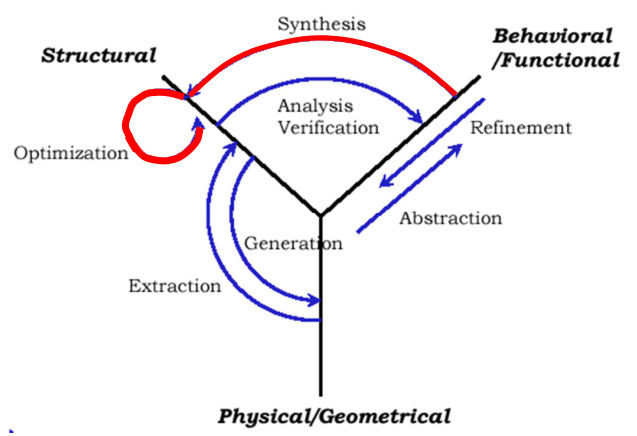
\includegraphics[height=70 mm]{./Cap1/Images/Image03.png}
	\caption[Optional caption]{Synthesis and Optimization}
	\label{fig:SynthOpt}
\end{figure}
\begin{flushleft}
	The \textbf{design} is the repetition of
\end{flushleft}
\begin{enumerate}
\item Modelling
\item Synthesis \& Optimization
\item Validation
\end{enumerate}
for each level: RTL, LOGIC, PHYSICAL.

\subsection{Design space}
The Design Space is where a dimension is a variable. The different feasible structural implementations of a circuit define its design space. The design space is a finite set of design points. Combined optimization of area (minimization) and performance (maximization) can be abstracted by representing the feasible structural implementations of a design into a design space.
\bigskip \\
\textbf{Optimization}: search an implementation that optimizes all
objectives.
\bigskip \\
A  point of the design space is called a  \textbf{Pareto point} if there is no other point (in the design space) with at least an inferior objective, all others being inferior or equal. A Pareto point corresponds to a global optimum in a monodimensional design evaluation space.\\ 
The image of the Pareto points in the design evaluation space is the set of the optimal  trade-off  points. Their interpolation yields a  trade-off curve  or  surface.
\begin{figure}[H]
	\centering
	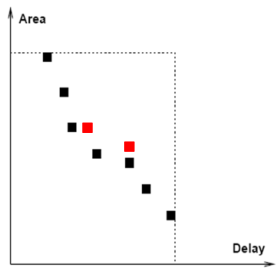
\includegraphics[height=50 mm]{./Cap1/Images/Image04.png}
	\caption[Optional caption]{Pareto Points}
	\label{fig:Pareto}
\end{figure}
\begin{flushleft}
	In the Figure \ref{fig:Pareto} the black points are the Pareto points.
\end{flushleft}

\subsection{General approaches to optimization}
Circuit optimization involves multiple objective functions. The optimization problem is difficult to solve, due to the discontinuous nature of the objective functions and to the discrete nature of the design space, i.e., of the set of feasible circuit implementations. In general, Pareto points  are  solutions to constrained optimization problems.\\
Consider, for example, \textit{logic-level} models. Then the following two problems are of interest:
\begin{itemize}
\item Minimize the circuit  \textit{area}  under  \textit{delay} constraints
\item Minimize the circuit  \textit{delay}  under  \textit{area} constraints
\end{itemize}
Unfortunately, due to the difficulty of the optimization problems, only approximations to the Pareto points can be computed.\\
Consider next \textit{architectural-level} models of synchronous circuits. Pareto points are solutions to the following problems, for different values of the \textbf{cycle-time}:
\begin{itemize}
\item Minimize the circuit \textit{area} under \textit{latency} constraints
\item Minimize the circuit \textit{latency} under \textit{area} constraints
\end{itemize}
These two problems are often referred to as \textit{scheduling problems}.

\cleardoublepage
\section{Modeling Languages and Abstract Models}

\subsection{HDL analysis}
A language can be characterized by its  syntax, semantics  and  pragmatics.\\
The \textit{syntax} relates to the language structure and it can be specified by a grammar.\\
The \textit{semantics} relates to the meaning of a language. The semantic rules associate actions to the language fragments that satisfy the syntax rules.\\
The \textit{pragmatics} relate to the other aspects of the language, including implementation issues. \\
Languages can be broadly classified as  procedural  and  declarative  languages. \textit{Procedural} programs specify the desired action by describing a sequence of steps whose order of execution matters. Conversely, \textit{declarative} models express the problem to be solved by a set of declarations without detailing a solution method. Therefore the order of the statements is not important in such languages.\\
Languages for hardware specification are classified on the basis of the description view that they support (e.g., physical, structural or behavioral).\\
Languages that support \textit{physical design} are characterized by having geometric primitives and by supporting operations on those primitives.\\
Models in \textit{structural languages} describe an interconnection of components. Hence their expressive power is similar to that of circuit schematics, even though specific language constructs can provide more powerful abstractions. Hierarchy is often used to make the description modular and compact.\\
Type of languages:
\begin{itemize}
\item Procedural languages: Specify the action (and so the circuit) by a sequence of steps (C, Pascal, VHDL, Verilog)
\item Declarative languages: Specify the hardware by a set of declaration (Logic netlist, VHDL, Verilog).
\end{itemize}
The success of VHDL and Verilog is due to at behavioral view it possible implement \textit{sequential} and \textit{combinational} descriptions.\\
Models in \textit{behavioral languages} can describe \textit{combinational} or \textit{sequential} circuits.\\
The \textit{combinational} circuit is described as a set of untimed assignment where each assignment represents a virtual logic gate (very similar to procedural models).\\
The sequential circuit is described throw declaration of \textit{Task}, use timing annotation for delayed signals. \\
The \textit{Tasks} can be, at architectural level, generic operations, or, at logic-level, logic functions.

\subsection{Abstract models}
A  model of a circuit is an abstraction, i.e., a representation that shows relevant features without associated details. Formal models have a well-defined syntax and semantics. Hence they provide a way of conveying the information about a circuit in a consistent way that can be unambiguously interpreted. Conversely, informal circuit specifications, such as textual descriptions have limited applications when  CAD  methods are used. In addition, informal descriptions of large-scale circuits or systems may be sources of misunderstanding among humans.\\
A circuit can be modelled differently according to the desired abstraction level (e.g., architectural, logic, geometric), view (e.g., behavioral, structural, physical) and the modelling means (e.g., language, diagram, mathematical model).\\
In recent years, there has been a trend toward using \textbf{hardware description languages} (HDLs) for circuit specification.\\
\textbf{Abstract models} are mathematical models based on graphs and Boolean algebra.\\
At the \textit{architectural level}, the circuit \textit{behavior} can be abstracted by a set of operations (called also tasks) and their dependencies. The operations can be general in nature, ranging from arithmetic to logic functions.\\
At the \textit{logic level}, the \textit{behavior} of a sequential logic circuit is abstracted by a finite-state machine that degenerates to a Boolean function in the  combinational case.\\
\textit{Structural views} are abstracted as interconnections of logic blocks or gates (at the logic level) or resources (at the architectural level).\\
Abstract models are powerful enough to capture the essential features described by HDL and diagram models. 
\begin{figure}[H]
	\centering
	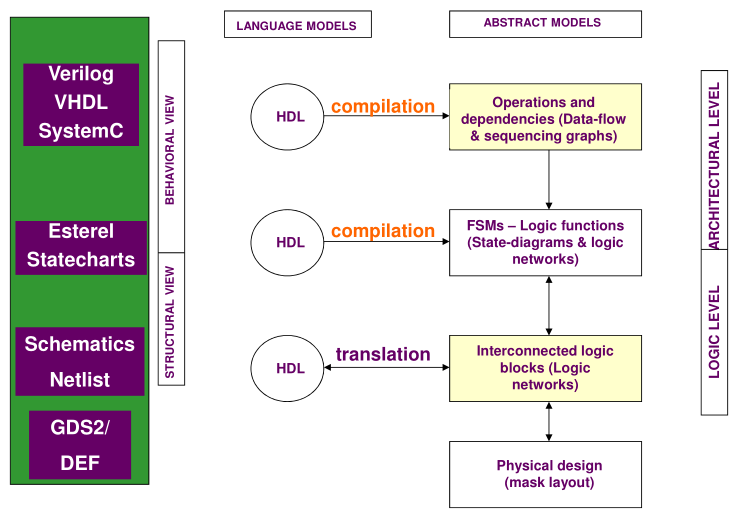
\includegraphics[height=100 mm]{./Cap2/Images/Image01.png}
	\caption[Optional caption]{Languages and abstract models}
	\label{fig:absMod}
\end{figure}
$ $\\[\spaceBreackLine]
Examples of \textbf{Abstract models}
\begin{itemize}
\item \textit{Logic networks}
\begin{itemize}
\item \textit{Mixed structural/behavioral views}
\item \textit{BDD} and \textit{AIG}
\end{itemize}
\item \textit{State diagrams}: The behavioral view of sequential circuits at the logic level can be expressed by finite-state machine transition diagrams
\item \textit{Dataflow} and \textit{sequencing graphs}
\end{itemize}

\subsubsection{Logic network (logic-level)}
A generalized \textit{logic network} is a structure, where each module is associated with a combinational or sequential logic function. Each block is modelled by a Boolean function. Each module is associated with a multiple-input, single-output combinational logic function, called a\textit{ local function}. Pins are partitioned into two classes, called \textit{input} and \textit{outputs}.
\subsubsection{Mixed structural/behavioral views}
In general, a logic network is a hybrid \textit{stmctural/behavioral representation}, because the the interconnections provide a structure while the logic functions denote the terminal behavior of the modules.
\begin{figure}[H]
    \centering
    \begin{subfigure}[b]{0.4\textwidth}
        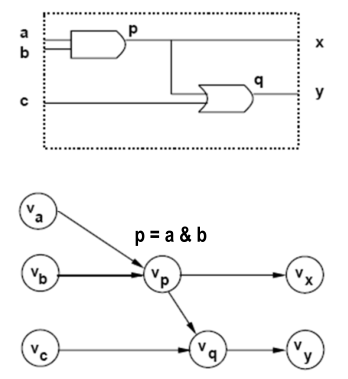
\includegraphics[width=\textwidth]{./Cap2/Images/Image02.png}
        \caption{Mapped network}
        \label{fig:map}
    \end{subfigure}
    \begin{subfigure}[b]{0.4\textwidth}
        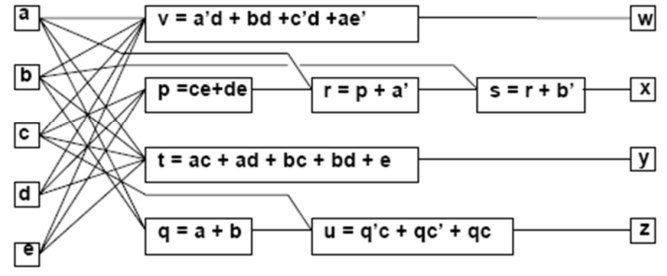
\includegraphics[width=\textwidth]{./Cap2/Images/Image03.png}
        \caption{General network}
        \label{fig:gen}
    \end{subfigure}
    \caption{Different networks}
    \label{fig:nets}
\end{figure}
The Figure \ref{fig:map} is a special case when the blocks correspond to \textit{library elements}.

\subsubsection{BDD (logic-level)}
A Binary Decision Diagram (BDD) is a directed acyclic graph (DAG)
\begin{itemize}
\item \textit{Graph}: set of vertices connected by edges
\item \textit{Directed}: edges have direction
\item \textit{Acyclic}: no path in the graph can lead to a cycle
\end{itemize}
Ordered BDD (\textbf{OBDD}):
\begin{enumerate}
\item Each vertex represents a decision on a variable
\item The value of the function is found at the leaves
\item Each path from root to leaf corresponds to a row in the truth table
\item Variables must appear in the same order along each path from root to leaves
\item Each variable can appear at most once on a path
\end{enumerate}
\begin{figure}[H]
    \centering
    \begin{subfigure}[b]{0.15\textwidth}
        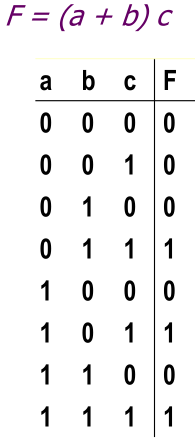
\includegraphics[width=\textwidth]{./Cap2/Images/Image04.png}
        \caption{True Table}
        \label{fig:trueTable}
    \end{subfigure}
    \quad\quad\quad
    \begin{subfigure}[b]{0.4\textwidth}
        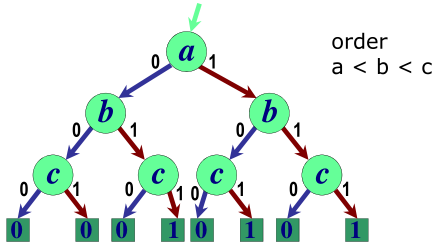
\includegraphics[width=\textwidth]{./Cap2/Images/Image05.png}
        \caption{OBDD}
        \label{fig:OBDD}
    \end{subfigure}
    \label{fig:OBDDs}
\end{figure}
The OBDD is a efficient way to represent logic functions. Each distinct function corresponds to a unique distinct diagram (\textit{Canonical form}). Efficient manipulation of Boolean functions, in fact many logical operations on OBDDs can be implemented in polynomial time (conjunction, negation, disjunction).\\
\textit{Drawbacks}: The size of a BDD is as big as a truth table.
\bigskip \\
The \textbf{Reduced OBDD} is obtained applying 2 roles:
\begin{enumerate}
\item Merging equivalent sub-trees
\item Removing nodes with identical children
\end{enumerate}

\subsubsection{AIG (logic-level)}
An And-Inverter Graph (AIG) is a  directed acyclic graph (DAG).
\textit{Nodes}:
\begin{itemize}
\item Terminal nodes representing variable names
\item Internal nodes representing AND function
\end{itemize}
\textit{Edge}: Those containing markers indicate logical negation.\\
AIG is fast, scalable (less memory) and with efficient manipulation. Each function can have different diagrams, it is not a \textit{Canonical form}.\\
The advantage of the AIG: the number of the leafs is equal to the number of the inputs (n) and not $ 2^{n} $ as in the ROBDD.
\begin{figure}[H]
	\centering
	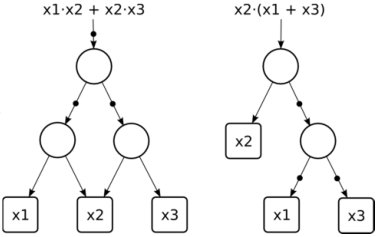
\includegraphics[height=50 mm]{./Cap2/Images/Image07.png}
	\caption[Optional caption]{Different Diagrams of the same function}
	\label{fig:aig}
\end{figure}
The Figure \ref{fig:aig} shows the AIG diagrams. Them must be read from the bottom to up.\\
Remember the \textit{Morgan's law}: $ \overline{x_{1} + x_{2}} = \overline{x_{1}} \overline{x_{2}} $\\
In the first diagram: $ \overline{\overline{x_{1} x_{2}} \, \overline{x_{2} x_{3}}} = x_{1} x_{2} + x_{2} x_{3} $

\subsubsection{State  Diagrams}
The behavioral view of sequential circuits at the logic level can be expressed by finite-state machine transition diagrams. A finite-state machine can be described by:
\begin{itemize}
\item A set of primary input panems, $X$
\item A set of primary output patterns, $Y$
\item A set of states, $S$
\item A \textit{state transition} function, $\delta : X \times S \rightarrow S$
\item An \textit{output function},  $\lambda :  X \times S \rightarrow Y $ for \textit{Mealy} models or  $\lambda : S \rightarrow Y $ for \textit{Moore}
\item An initial state
\end{itemize}
The \textit{state transition table} is a tabulation of the state transition and output functions. Its corresponding graph-based representation is the \textit{state transition diagram}.
\begin{figure}[H]
	\centering
	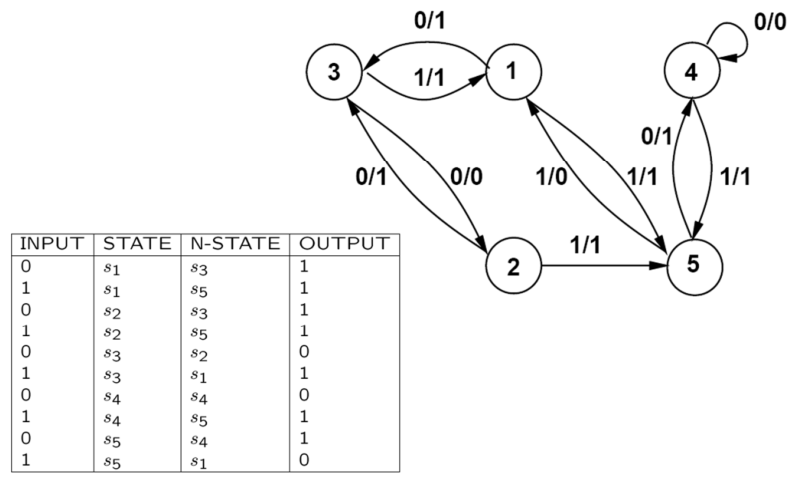
\includegraphics[height=45 mm]{./Cap2/Images/Image06.png}
	\caption[Optional caption]{State transition table and state transition diagram}
	\label{fig:stateDia}
\end{figure}

\subsubsection{Dataflow graphs – DFG (Architectural-level)}
We consider here models that abstract the information represented by procedural HDLs. Abstract models of behavior at the architectural level are in terms of  \textit{operations}  (Vertices)  and their  \textit{dependencies} (Edges).
\begin{figure}[H]
	\centering
	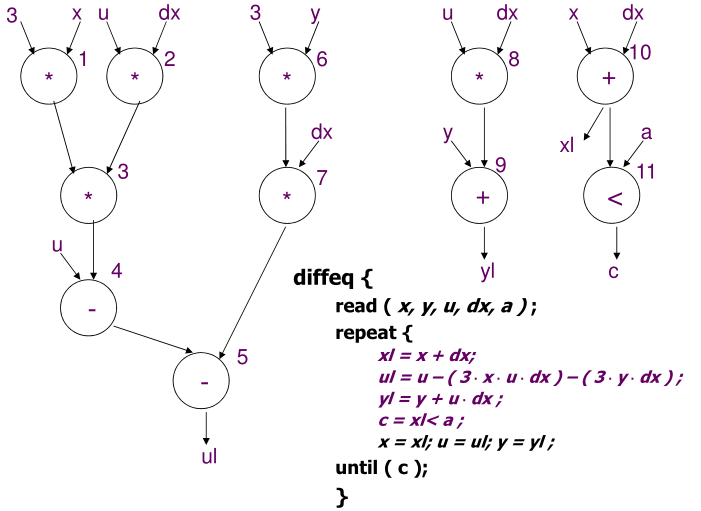
\includegraphics[height=45 mm]{./Cap2/Images/Image08.png}
	\caption[Optional caption]{DFG}
	\label{fig:DFG}
\end{figure}
Control-flow information, related to  \textit{branching}  (or  \textit{conditional})  and  \textit{iteration} (or  \textit{loop})  constructs, can also be represented graphically. Many different models have been proposed to represent \textit{control/data-flow graphs}.\\
The simplest approach is to extend further data-flow graphs by introducing branching vertices that represent operations that evaluate conditional clauses.  A  \textit{branching} vertex is the tail of a set of alternative paths, corresponding to the possible branches. \textit{Iteration} can be modelled as a branch based on the iteration exit condition. The corresponding vertex is the tail of two edges, one modelling the exit from the loop and the other the return to the first operation in the loop.\\
One particular abstract model for tasks subject to data- and control-flow dependencies is called \textit{sequencing graph}. It is a hierarchical control/data-flow graph, where control-flow primitives such as branching and iteration are modelled through the hierarchy, whereas data-flow and serialization dependencies are modelled by graphs. In addition, the hierarchical model supports a  model call,  i.e., the encapsulation of subsets of operations and their dependencies into blocks that can be multiply invoked.\\
The graph has two major properties:
\begin{itemize}
\item Acyclic
\item Polar: there are two vertices, called  \textit{source}  and  \textit{sink},  that represent the first and last tasks.
\end{itemize}
\begin{figure}[H]
    \centering
    \begin{subfigure}[b]{0.2\textwidth}
        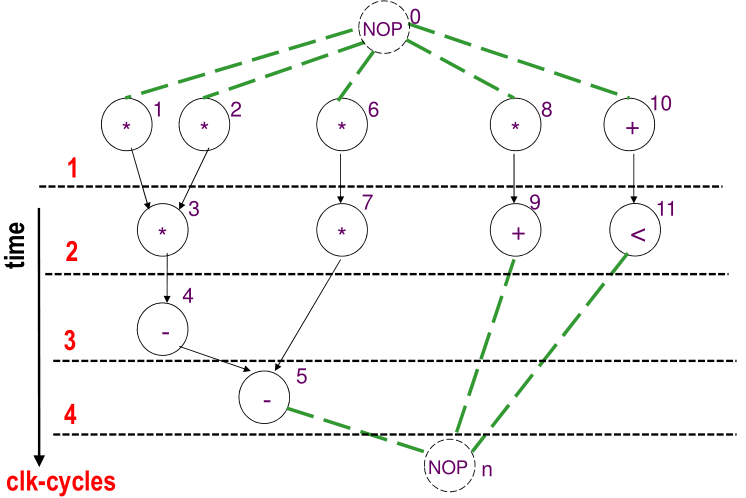
\includegraphics[width=\textwidth]{./Cap2/Images/Image09.png}
        \caption{Sequencing DFG}
        \label{fig:SequencingDFG}
    \end{subfigure}
    \quad
    \begin{subfigure}[b]{0.2\textwidth}
        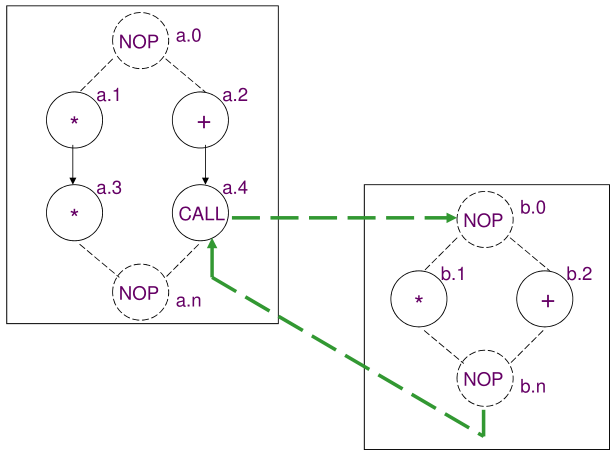
\includegraphics[width=\textwidth]{./Cap2/Images/Image10.png}
        \caption{Hierarchy DFG}
        \label{fig:HierarchyDFG}
    \end{subfigure}
    \quad
    \begin{subfigure}[b]{0.2\textwidth}
        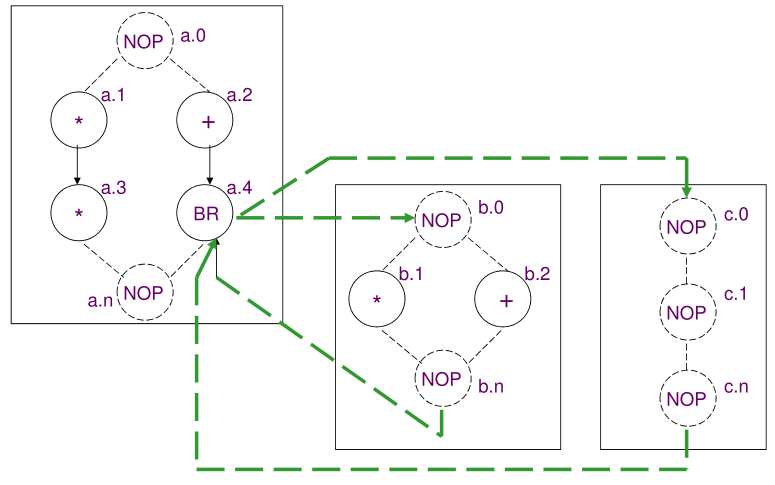
\includegraphics[width=\textwidth]{./Cap2/Images/Image11.png}
        \caption{Branching DFG}
        \label{fig:BranchingDFG}
    \end{subfigure}
    \quad
    \begin{subfigure}[b]{0.2\textwidth}
        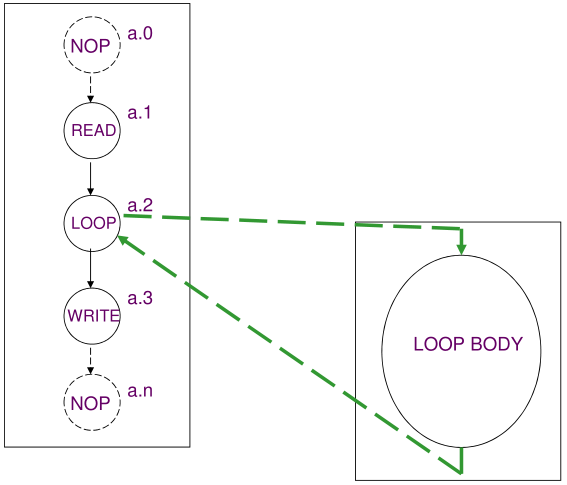
\includegraphics[width=\textwidth]{./Cap2/Images/Image12.png}
        \caption{Iteration DFG}
        \label{fig:IterationDFG}
    \end{subfigure}
    \label{fig:DFGs}
    \caption{Different examples of DFG}
\end{figure}
Some attributes can be assigned to the vertices and edges of a sequencing graph model, such as measures or estimates of the corresponding \textit{area} or delay \textit{cost}. In general, the delay of  a  vertex can be  data independent  or  data dependent.  Only data-independent delays can be estimated before synthesis. An example data-dependent iteration is given by an arithmetic divisor, based on an iterative algorithm. Data-dependent delays can be  \textit{bounded}  or  \textit{unbounded}.  The former case applies to data-dependent delay branching, where the maximum and minimum possible delays can be computed. The latter case is typical of some other iteration constructs.
\cleardoublepage
\section{Architectural-Level Synthesis}
Trying to pass from logic to architectural level racecourse at higher level allow to see all possible options. Having less details, it possible work with higher complex circuit. You can decide to use a bigger block with high complexity at logic level, but the block that you have connected and improved don't allow to see a global improvement.\\
The motivations to raise abstraction level:
\begin{itemize}
\item Reduce specification of details
\item Extend designer base
\item Ease modifications and extensions
\item Reduce design time
\item Explore and optimize macroscopic structure
\end{itemize}
Architectural synthesis means constructing the macroscopic structure of a digital circuit, starting from behavioral models that can be captured by data-flow or sequencing graphs. The outcome of architectural synthesis is both a structural view of the circuit, in particular of its data path, and a logic-level specification of its control unit. The data path is an interconnection of  \textit{resources} (implementing arithmetic or logic functions), \textit{steering logic circuits}  (e.g., multiplexers and buses), that send data to the appropriate destination at the appropriate time and  \textit{registers}  or  \textit{memory arrays}  to store data.
\begin{figure}[H]
	 \centering
	 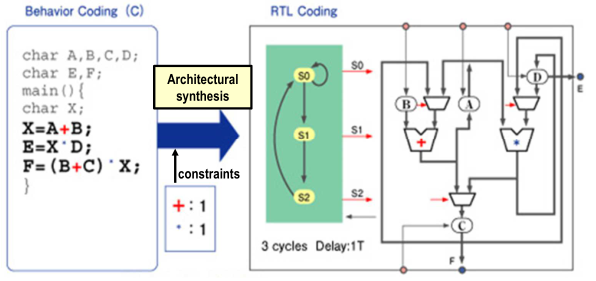
\includegraphics[height=50mm]{./Cap3/Images/Image01.png}
	 \caption[Optional caption]{Example of Architectural synthesis}
	 \label{fig:archSy}
\end{figure}

\subsection{Hardware and software compilation}
A \textit{software} compiler consists of a  front end  that transforms a program into an intermediate form  and a  back end  that translates the intermediate form into the machine code for a given architecture. The front end is language dependent, and the back end varies according to the target machine. Similarly, a \textit{hardware} compiler can be seen as consisting of a front end, an optimizer and a back end (Figure 3.16). The back end is much more complex than a software compiler, because of the requirements on timing and interface of the internal
operations.
\begin{figure}[H]
	 \centering
	 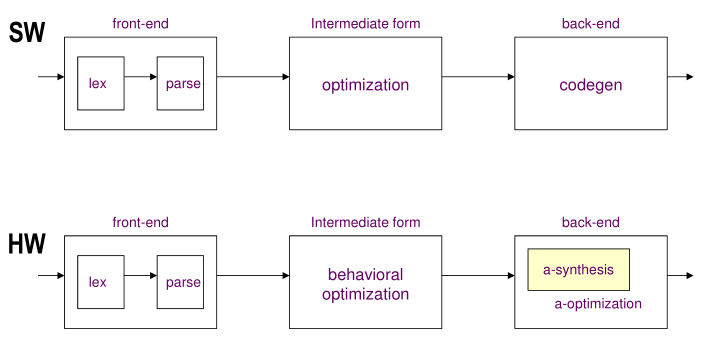
\includegraphics[height=50mm]{./Cap3/Images/Image02.png}
	 \caption[Optional caption]{Hardware and software compilation}
	 \label{fig:comp}
\end{figure}

\subsubsection{Compilation  Techniques}
The front end of a compiler is responsible for  \textit{lexical}  and  \textit{syntax} analysis, \textit{parsing}  and \textit{creation} of the intermediate form. Its first task is to verify that they satisfy the syntax rules of the language. The parser has knowledge of the grammar of the language and it generates a set of  parse trees.  A parse tree is a tree-like representation of the syntactic structure of a language. An example is shown in Figure \ref{fig:parseTree}. Syntactic errors, as well as some semantic errors are detected at this stage.
\begin{figure}[H]
	 \centering
	 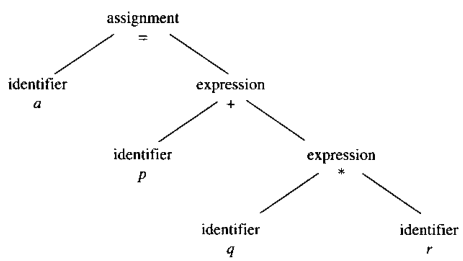
\includegraphics[height=50mm]{./Cap3/Images/Image03.png}
	 \caption[Optional caption]{Example  of  a  parse  tree  for  the statement  $ a  =  p  +  y  *  r $}
	 \label{fig:parseTree}
\end{figure}
Branching constructs can be used to model logic networks. A common way to exploit branching is by means of conditional assignments to a variable.  A  branching construct can be replaced by one logic expression, representing the disjunction of the possible assignments in conjunction with the test on the clause. When the branching construct does not specify an assignment for all values of the clause, the missing assignments represent  \textit{don't  care}  conditions on that variable. The compilation of hardware models at the architectural level involves a full \textit{semantic}, \textit{analyses}  that comprises  \textit{data-flow}  and  \textit{control-flow}  analyses.
\begin{figure}[H]
	 \centering
	 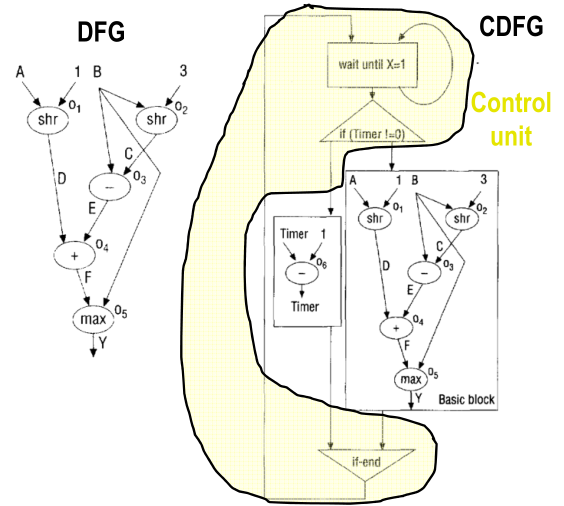
\includegraphics[height=50mm]{./Cap3/Images/Image04.png}
	 \caption[Optional caption]{Data-flow graph and Control-data-flow graph}
	 \label{fig:dataFlow}
\end{figure}

\subsubsection{Optimization Techniques}
Behavioral optimization is a set of transformations that minimize the amount of information needed to specify the partial order of tasks. It can be applied directly to the parse trees, or during the generation of the intermediate form.\\
Algorithms for behavioral optimization of  HDL  models can he classified as data-flow and control-flow
oriented.
\begin{itemize}
\item \textbf{DATA-FLOW-BASED TRANSFORMATIONS}: 
	\begin{itemize}
	\item \textit{Tree-height reduction}: This transformation applies to the arithmetic expression trees and strives to achieve the expression split into two-operand expressions, so that the parallelism available in hardware can be exploited at best. The simplest reduction algorithm uses the \textit{commutativity} and \textit{associativity} of the addition and multiplication. It permutes the operands to achieve subexpressions involving the same operator, which can be reduced by using the associative property. A  further refinement can be achieved by exploiting the \textit{distributive} property, possibly at the expense of adding an operation.
	\begin{figure}[H]
    \centering
    \begin{subfigure}[b]{0.4\textwidth}
        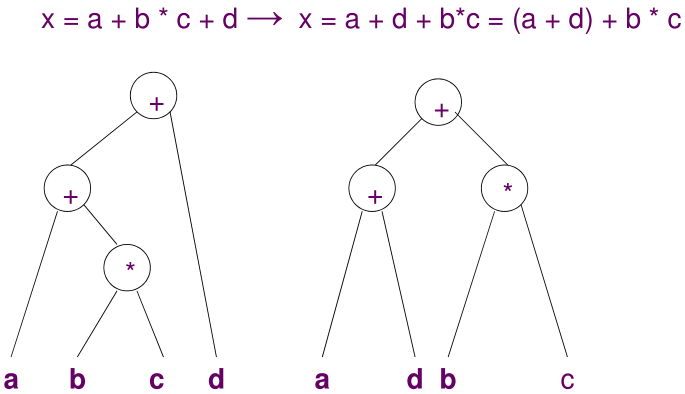
\includegraphics[width=\textwidth]{./Cap3/Images/Image05.png}
        \caption{using Commutativity and Associativity}
        \label{fig:comAss}
    \end{subfigure}
    \quad\quad\quad
    \begin{subfigure}[b]{0.4\textwidth}
        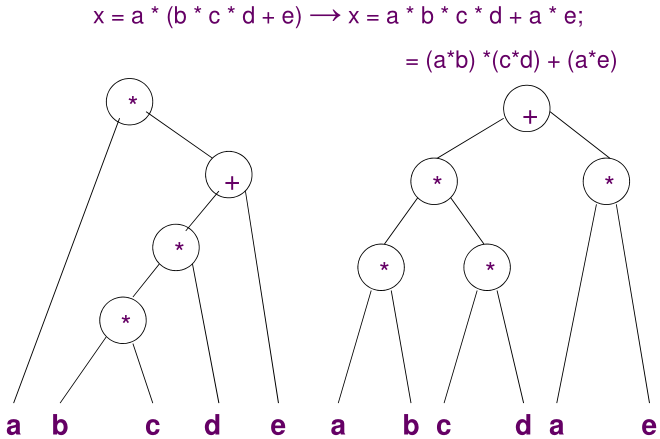
\includegraphics[width=\textwidth]{./Cap3/Images/Image06.png}
        \caption{using Distributivity}
        \label{fig:Dis}
    \end{subfigure}
	\end{figure}
	\item \textit{constant and variable propagation}:  \textit{Constant} propagation consists of detecting constant operands and pre-computing the value of the operation with that operand. Since the result may be again a constant, the new constant can be propagated to those operations that use it as input.
	\begin{figure}[H]
	 \centering
	 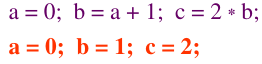
\includegraphics[width=0.25\textwidth]{./Cap3/Images/Image07.png}
	\end{figure}
	\textit{Variable} propagation consists of detecting the copies  of variables, i.e., the assignments like  x  =  y,  and using the right-hand side in the following references in place of the left-hand side. 
	\begin{figure}[H]
	 \centering
	 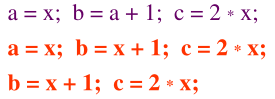
\includegraphics[width=0.25\textwidth]{./Cap3/Images/Image08.png}
	\end{figure}
	\item \textit{Common subexpression elimination}: The search for common arithmetic subexpressions relies in general on finding isomolphic patterns in the parse trees (\textit{Isomorphic}: if the subtree has the same inputs and the same operators). This step is greatly simplified if the arithmetic expressions are reduced to two-input ones. Then, this transformation consists of selecting a target arithmetic operation and searching for a preceding one of the same type and with the same operands.
	\begin{figure}[H]
	 \centering
	 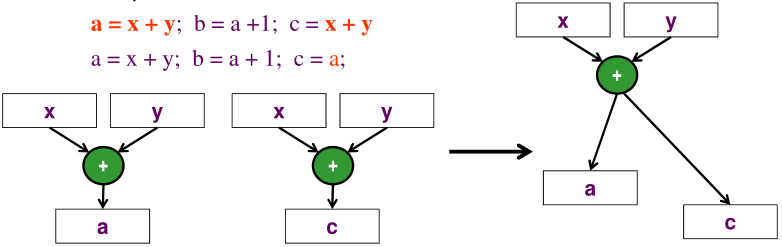
\includegraphics[width=0.4\textwidth]{./Cap3/Images/Image09.png}
	\end{figure}
	\item \textit{Dead code elimination};  Dead code consists of all those operations that cannot be reached, or whose result is never referenced elsewhere. 
	\begin{figure}[H]
	 \centering
	 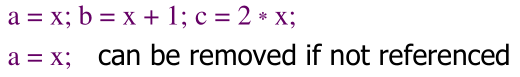
\includegraphics[width=0.4\textwidth]{./Cap3/Images/Image10.png}
	\end{figure}
	\item \textit{Operator strength reduction}:  Operator strength reduction means reducing the cost of implementing an operator by using a simpler one. 
	\begin{figure}[H]
	 \centering
	 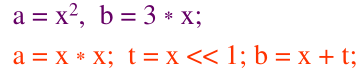
\includegraphics[width=0.3\textwidth]{./Cap3/Images/Image11.png}
	\end{figure}
	\item \textit{Code motion}:  Code motion often applies to loop invariants, i.e., quantities that are computed inside an iterative construct but whose values do not change from iteration to iteration. The goal is to avoid the repetitive evaluation of the same expression.
	\begin{figure}[H]
	 \centering
	 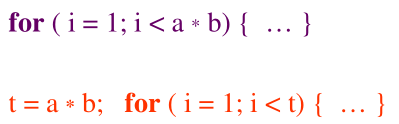
\includegraphics[width=0.3\textwidth]{./Cap3/Images/Image12.png}
	\end{figure}
	\end{itemize}
\item \textbf{CONTROL-FLOW-BASED TRANSFORMATIONS}:  The following transformations are typical of hardware compilers. In some cases these transformations are automated, in others they are user driven.
	\begin{itemize}
	\item \textit{Model expansion}: Consists in flattening locally the model call hierarchy. Therefore the called model disappears, being swallowed by the calling one. A  possible benefit is that the scope of application of some optimization techniques  is enlarged.
	\begin{figure}[H]
	 \centering
	 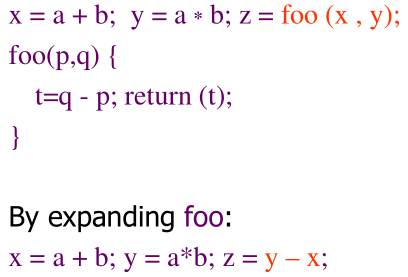
\includegraphics[width=0.3\textwidth]{./Cap3/Images/Image13.png}
	\end{figure}
	\item \textit{Conditional expansion}:  A  conditional construct can be always transformed into a parallel construct with a test in the end. Under some circumstances this transformation can increase the performance of the circuit. 
	\begin{figure}[H]
	 \centering
	 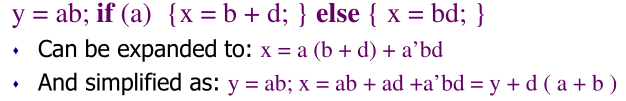
\includegraphics[width=0.5\textwidth]{./Cap3/Images/Image14.png}
	\end{figure}
	\item \textit{Loop expansion}:  Loop expansion, or unrolling, applies to an iterative construct with data-independent exit conditions. The loop is replaced by as many instances of its body as the number of operations. The benefit is again in expanding the scope of other transformations. 
	\begin{figure}[H]
	 \centering
	 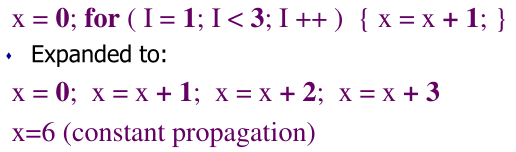
\includegraphics[width=0.4\textwidth]{./Cap3/Images/Image15.png}
	\end{figure}
	\end{itemize}
\end{itemize}

\subsection{Architectural synthesis and optimization}


	
\end{document}